\begin{figure*}[htbp]
    \centering
    \begin{tabular}{m{77mm} m{77mm} m{10mm}}
        \begin{minipage}[b]{\linewidth}
            \centering
            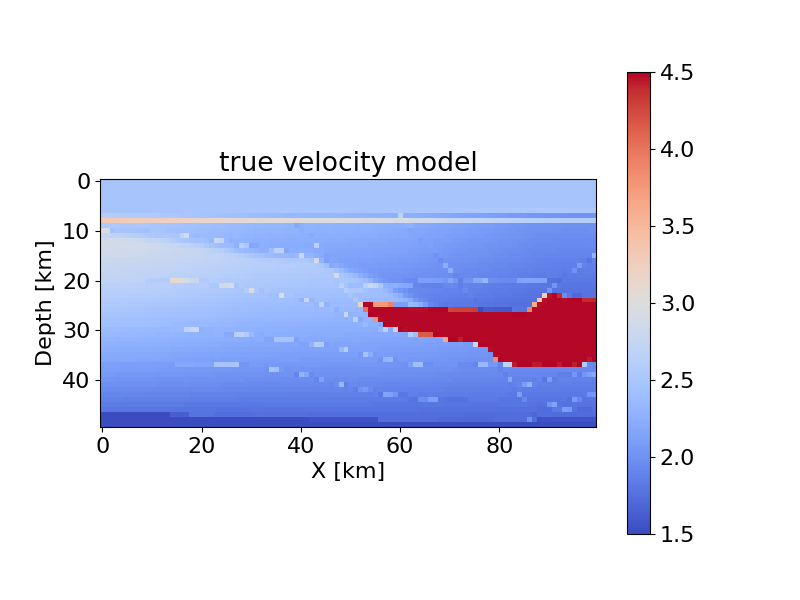
\includegraphics[width=\linewidth]{public/true}
            \vspace{-7mm}
            \caption*{\raisebox{2mm}{Ground truth}}
            \vspace{1mm}
        \end{minipage} &
        \begin{minipage}[b]{\linewidth}
            \centering
            
\includegraphics[width=\linewidth]{public/initial}
            \vspace{-7mm}
            \caption*{\raisebox{2mm}{Initial model}}
            \vspace{1mm}
        \end{minipage} &
        \multirow[t]{3}{*}{\raisebox{-104mm}{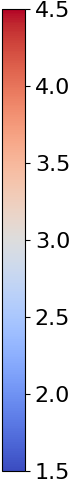
\includegraphics[height=70mm]{public/color-bar}}} \\

        \begin{minipage}[b]{\linewidth}
            \centering
            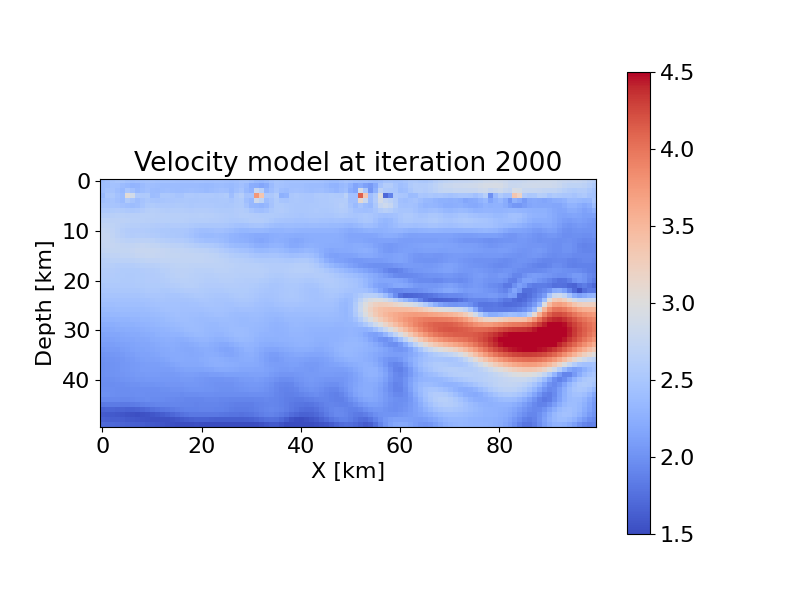
\includegraphics[width=\linewidth]{public/gradient}
            \vspace{-7mm}
            \caption*{\raisebox{2mm}{The Standard FWI Method}}
            \vspace{1mm}
        \end{minipage} &
        \begin{minipage}[b]{\linewidth}
            \centering
            \vspace{-2mm}
            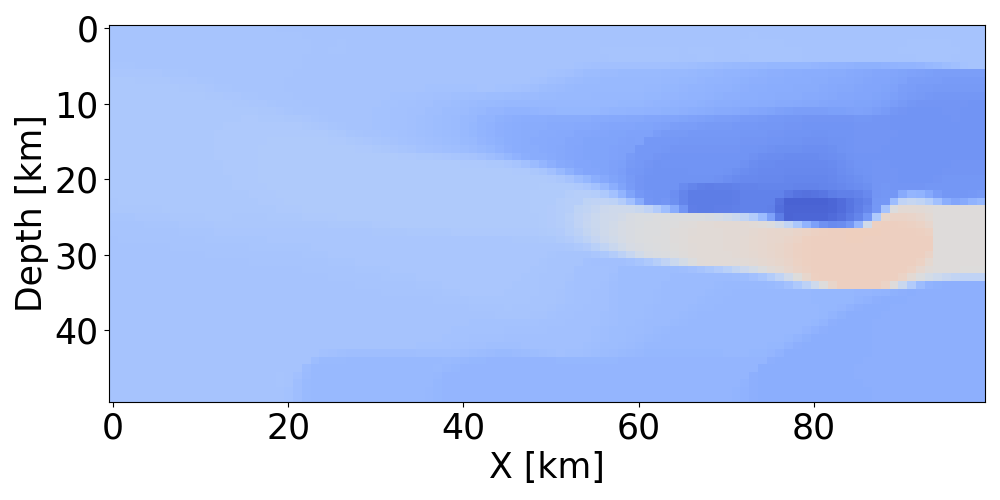
\includegraphics[width=\linewidth]{public/alpha_150}
            \vspace{-9mm}
            \caption*{Proposed Method, $\alpha = 150$}
            \vspace{1mm}
        \end{minipage} \\

        \begin{minipage}[b]{\linewidth}
            \centering
            \vspace{-1mm}
            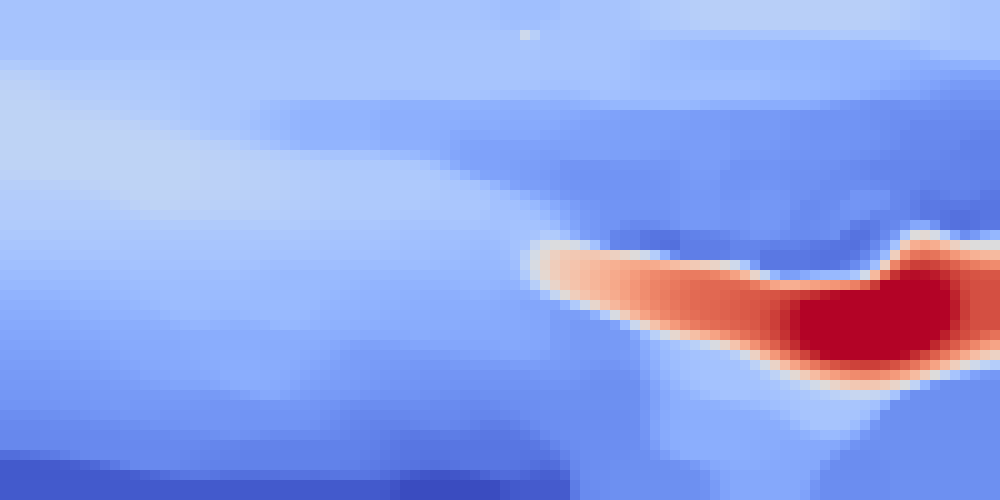
\includegraphics[width=\linewidth]{public/alpha_350}
            \vspace{-8mm}
            \caption*{Proposed Method, $\alpha = 350$}
            \vspace{1mm}
        \end{minipage} &
        \begin{minipage}[b]{\linewidth}
            \centering
            \vspace{-1mm}
            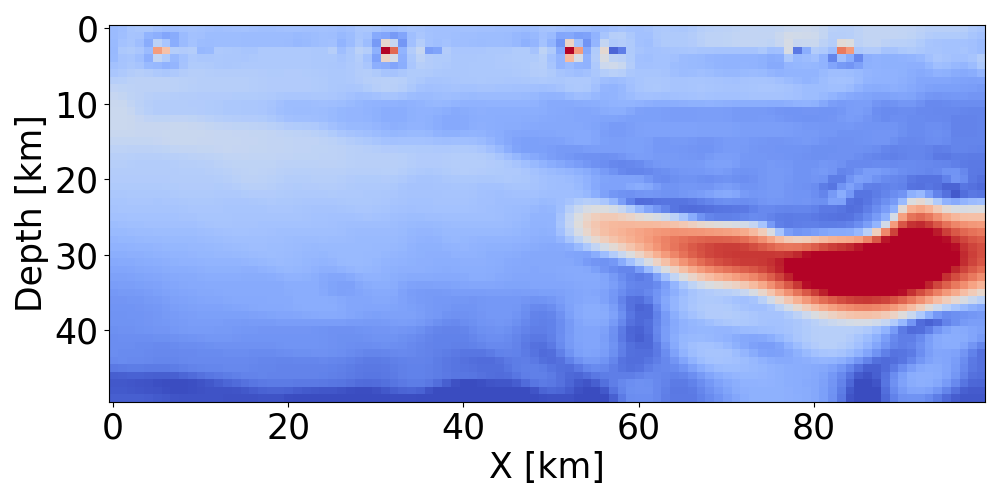
\includegraphics[width=\linewidth]{public/alpha_550}
            \vspace{-8mm}
            \caption*{Proposed Method, $\alpha = 550$}
            \vspace{1mm}
        \end{minipage} &
    \end{tabular}
    \caption{Velocity models [km/s] and their corresponding reconstructions.}
    \label{fig:velocity-models}
\end{figure*}


\subsection{Experimental Setup} \label{subsec:experimental-setup}

To demonstrate the effectiveness of the TV and box constrained FWI, we conducted FWI experiments where we compared with the standard FWI method\footnote{
    The standard FWI method uses the following procedures:
    \begin{equation} \label{eq:FWIWithGradient} \FWIWithGradient, \end{equation} where $\gamma$ is the step size.
}\cite{FWI0}, using the SEG/EAGE Salt and Overthrust Models.

The velocity model consists of 51 $\times$ 101 grid points.
The ground truth velocity model is generated by zooming and cropping Fig.~\ref{fig:salt-model}.
The initial velocity model is generated by smoothing the ground truth velocity model with a Gaussian function with a standard deviation of 80.
The source waveform is a Ricker wavelet with a peak wavelet frequency of 10 Hz.
The number of waveform sources and receivers is 20 and 101, respectively, and they are placed on the surface at equal intervals.
The gradient $\nabla E$ is computed numerically using the Devito framework\cite{devito}.
The number of iterations is set to 5000.
In our algorithm, the step sizes $\gamma_1$ and $\gamma_2$ are set to $1.0 \times 10^{-4}$ and $1.0 \times 10^2$, respectively.
The lower and upper bounds of the velocity model $l$, $u$ are set to 1.5[km/s] and 4.5[km/s], respectively.
The experiments are conducted using $\alpha$ values ranging from 100 to 700 in steps of 50, representing the upper bound of the $l_{1,2}$ norm.
In the standard FWI method, the step size $\gamma$ is set to $1.0 \times 10^{-4}$.

\begin{figure*}[htbp]
    \centering
    \hspace{-3mm}
%    \begin{minipage}{58mm}
%        \centering
%        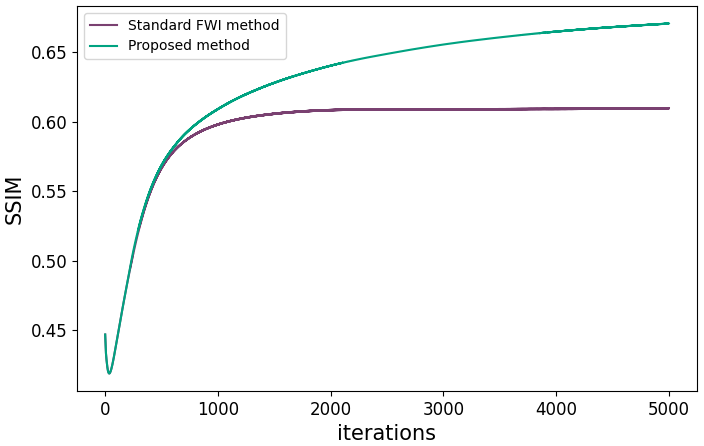
\includegraphics[width=\linewidth]{public/iters-ssim}
%%        \vspace{-6mm}
%        \caption{SSIM against iters.}
%        \label{fig:iters-ssim}
%        \vspace{-2mm}
%    \end{minipage}
%    \hspace{-1mm}
    \begin{minipage}{58mm}
        \centering
        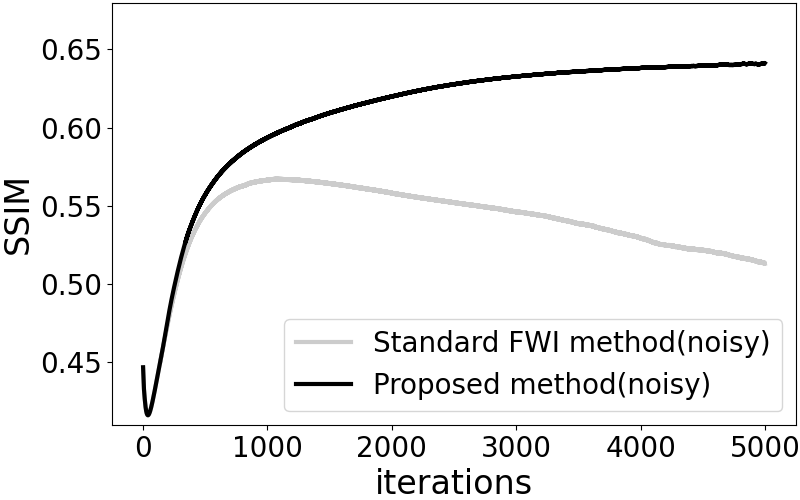
\includegraphics[width=\linewidth]{public/iters-ssim-noisy}
%        \vspace{-6mm}
        \caption{SSIM against iters. (noisy)}
        \label{fig:iters-ssim-noisy}
        \vspace{-3mm}
    \end{minipage}
    \hspace{-1mm}
    \begin{minipage}{58mm}
        \centering
        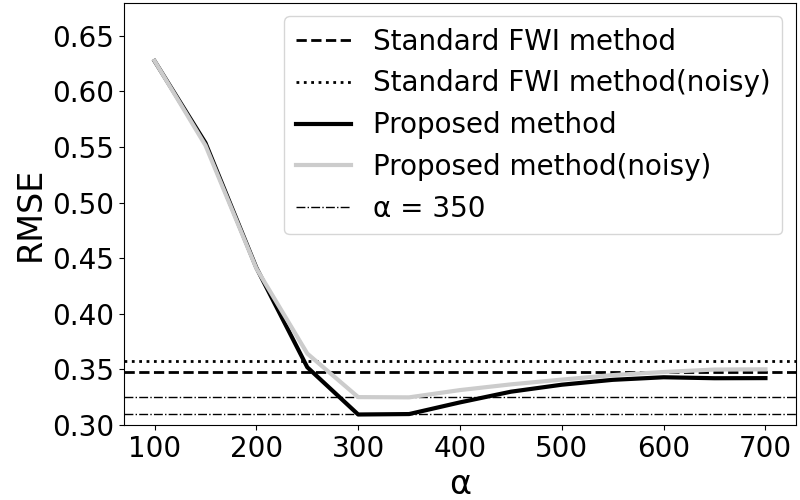
\includegraphics[width=\linewidth]{public/alpha-rmse-edited}
%        \vspace{-6mm}
        \caption{RMSE against $\alpha$.}
        \label{fig:alpha-rmse}
        \vspace{-3mm}
    \end{minipage}
    \hspace{-2mm}
    \begin{minipage}{58mm}
        \centering
        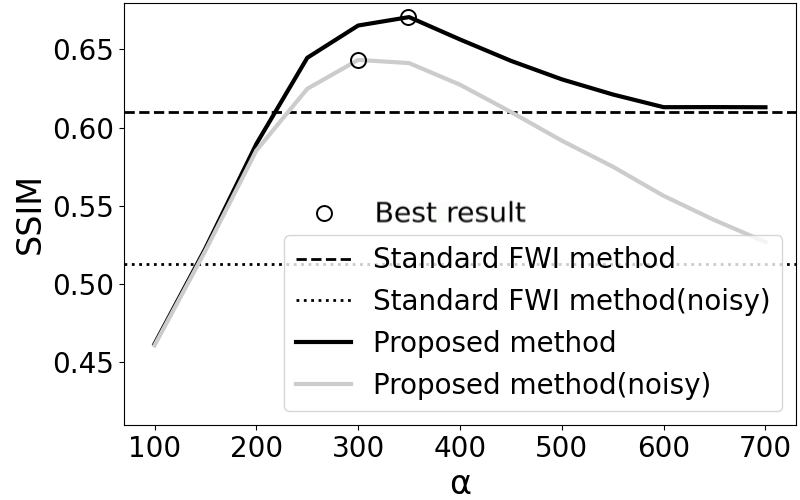
\includegraphics[width=\linewidth]{public/alpha-ssim-all-edited}
%        \vspace{-6mm}
        \caption{SSIM against $\alpha$.}
        \label{fig:alpha-ssim}
        \vspace{-3mm}
    \end{minipage}
\end{figure*}




\subsection{Results and Discussion} \label{subsec:results-and-discussion}

Fig.~\ref{fig:velocity-models} shows the ground truth, the initial model, and the reconstructed velocity models using the standard FWI method and the proposed methods with $\alpha$ = 150, 350, and 550.
The best parameter is $\alpha$ = 350, where $\alpha$ = 150 represents a stronger TV constraint and $\alpha$ = 550 represents a weaker one.
The standard FWI method generates wave-like artifacts and noise around the source positions.
In contrast, our proposed method with the best parameter achieves the accurate velocity model reconstruction without these artifacts and noise.
When the TV constraint is too strong, as with $\alpha$ = 150, over-smoothing occurs, reducing contrast in the reconstruction.
On the other hand, when the TV constraint is too weak, as with $\alpha$ = 550, the constraint has little effect, leading to results similar to those of the standard FWI method.

For quantitative evaluation, we plot the Structural Similarity Index Measure (SSIM) against the number of iterations for our proposed method and the standard FWI method in Fig.~\ref{fig:iters-ssim}.
The proposed method consistently achieves higher SSIM values than the standard FWI method at every iteration, indicating enhanced reconstruction accuracy.

For a more detailed analysis of the TV constraint parameter $\alpha$, we plot the SSIM of our proposed method against the parameter $\alpha$ and the standard FWI method in Fig.~\ref{fig:alpha-ssim}.
As mentioned earlier, at $\alpha$ = 350, the proposed method achieves the highest SSIM.
As $\alpha$ is smaller, meaning the TV constraint becomes stronger, the SSIM worsens.
On the other hand, when $\alpha$ becomes too large, the SSIM of our proposed method resemble that of standard FWI method.
However, thanks to the box constraint, the proposed method still outperforms the standard FWI method.
This demonstrates that the parameter $\alpha$ has a clear and predictable effect on the reconstructed velocity model, which can be easily adjusted to achieve accurate results
